\documentclass[a4paper,12pt]{article}

\usepackage{graphicx}
\graphicspath{ {./images/} }
\usepackage{amsmath}
\usepackage{hyperref}
\usepackage{listings}
\usepackage{xcolor}
\usepackage{geometry}
\geometry{a4paper, margin=1in}

% Define code listing style
\lstset{
    basicstyle=\ttfamily\footnotesize,
    backgroundcolor=\color{gray!10},
    frame=single,
    breaklines=true,
    keywordstyle=\color{blue},
    commentstyle=\color{green!50!black},
    stringstyle=\color{red!50!brown},
    showstringspaces=false
}

\title{Deep Q-Learning for Flappy Bird: Implementation and Evaluation}
\author{Rusu Andrei-Dudu, Zloteanu Mircea}
\date{January 4, 2025}

\begin{document}

\maketitle

\begin{abstract}
This report presents the implementation and evaluation of a Deep Q-Learning (DQN) agent trained to play Flappy Bird using PyTorch and Gymnasium. The report details the neural network architecture, hyperparameter settings, and experimental results. Various training runs were conducted to evaluate the performance of the agent under different configurations. The best-performing agent achieved a maximum score of \textbf{763} across multiple runs.
\end{abstract}

\section{Introduction}
Flappy Bird is a challenging and fast-paced game, making it an ideal testbed for reinforcement learning algorithms. This project leverages the Deep Q-Learning algorithm with experience replay and a convolutional neural network (CNN) to approximate Q-values. The goal is to train an agent capable of achieving a high score consistently.

\section{Methodology}

\subsection{Agent Architecture}
The DQN agent consists of two main components:
\begin{enumerate}
    \item \textbf{Neural Network (NN)}: The network is designed to approximate Q-values for each action using convolutional and fully connected layers:
    \begin{itemize}
        \item \textbf{Input Layer}: Grayscale image of size \(84 \times 84\).
        \item \textbf{Convolutional Layers}:
        \begin{itemize}
            \item Layer 1: \(1 \rightarrow 32\) channels, kernel size \(3 \times 3\), stride 1, padding 1.
            \item Layer 2: \(32 \rightarrow 64\) channels, kernel size \(3 \times 3\), stride 1, padding 1.
            \item Layer 3: \(64 \rightarrow 128\) channels, kernel size \(3 \times 3\), stride 1, padding 1.
            \item Layer 4: \(128 \rightarrow 256\) channels, kernel size \(3 \times 3\), stride 1, padding 1.
        \end{itemize}
        \item \textbf{Fully Connected Layers}:
        \begin{itemize}
            \item Flatten layer: Output from convolutional layers flattened to \(256 \times 5 \times 5\).
            \item Dense Layer 1: \(256 \times 5 \times 5 \rightarrow 512\) units.
            \item Output Layer: \(512 \rightarrow 2\) (Q-values for actions).
        \end{itemize}
    \end{itemize}
    \item \textbf{Replay Buffer}: A fixed-size replay buffer stores past experiences for sampling during training.
\end{enumerate}

\subsection{Hyperparameters}
The training hyperparameters used for the DQN agent are summarized in Table~\ref{tab:hyperparameters}.
\begin{table}[!ht]
\centering
\begin{tabular}{|l|c|}
\hline
\textbf{Parameter}           & \textbf{Value}          \\ \hline
Learning Rate (\(\eta\))     & \(1 \times 10^{-5}\)     \\ \hline
Discount Factor (\(\gamma\)) & \(0.99\)                \\ \hline
Epsilon (\(\epsilon\))       & \(0.1 \rightarrow 0.0001\) (decay 0.995) \\ \hline
Batch Size                   & 32                      \\ \hline
Replay Buffer Capacity       & 50,000                  \\ \hline
Training Start Threshold     & 5,000 experiences       \\ \hline
Number of Epochs             & 2,000                   \\ \hline
\end{tabular}
\caption{Hyperparameters for training the DQN agent.}
\label{tab:hyperparameters}
\end{table}

\subsection{Explanation of Hyperparameters}
The hyperparameters used in training the DQN agent play a crucial role in determining its performance. Below is a detailed explanation of each parameter:

\begin{itemize}
    \item \textbf{Learning Rate (\(\eta\))}: A small learning rate of \(1 \times 10^{-5}\) ensures that the updates to the neural network weights are gradual, reducing the risk of overshooting the optimal values during training.

    \item \textbf{Discount Factor (\(\gamma\))}: The discount factor of \(0.99\) prioritizes long-term rewards, helping the agent to plan strategies over multiple steps instead of focusing solely on immediate gains.

    \item \textbf{Epsilon (\(\epsilon\))}: 
    Initially set to \(0.1\), epsilon facilitates exploration by encouraging the agent to take random actions. Over time, it decays to \(0.0001\) with a decay rate of \(0.995\), shifting the agent's behavior towards exploitation of its learned policy.

    \item \textbf{Batch Size}: A batch size of 32 ensures computational efficiency while maintaining sufficient diversity in the training samples, improving the robustness of updates to the neural network.

    \item \textbf{Replay Buffer Capacity}: The replay buffer holds up to 50,000 experiences, providing a diverse set of past interactions for training. This helps to reduce temporal correlations in the data, stabilizing the learning process.

    \item \textbf{Training Threshold}: The agent begins training only after 5,000 experiences are collected in the replay buffer. This ensures a diverse set of data is available, preventing premature updates that could hinder learning.

    \item \textbf{Number of Epochs}: Training the agent over 2,000 epochs allows sufficient iterations for the neural network to learn and adapt to the environment, achieving stable performance.

\end{itemize}

These carefully chosen hyperparameters ensure that the agent learns effectively while balancing exploration and exploitation. The use of a replay buffer and batch sampling further contributes to stable and efficient training.

\subsection{Preprocessing}
The input images undergo the following preprocessing steps:
\begin{enumerate}
    \item Crop the bottom 110 pixels to remove irrelevant information.
    \item Convert the cropped image to grayscale.
    \item Resize to \(84 \times 84\) pixels.
    \item Normalize pixel values to \([0, 1]\) and convert to tensors.
\end{enumerate}

\subsection{Training Procedure}
The training process consists of:
\begin{enumerate}
    \item Epsilon-greedy action selection.
    \item Experience replay with randomly sampled mini-batches.
    \item Q-value updates using the Bellman equation.
    \item Saving model checkpoints every 100 epochs.
\end{enumerate}

\section{Implementation Details}
\subsection{Q-Learning Algorithm}
The Q-learning algorithm uses the Bellman equation to update the Q-values:
\[
Q(s, a) \leftarrow Q(s, a) + \alpha \Big( r + \gamma \max_{a'} Q(s', a') - Q(s, a) \Big)
\]
where:
\begin{itemize}
    \item \(s\) and \(s'\) are the current and next states.
    \item \(a\) and \(a'\) are the current and next actions.
    \item \(r\) is the reward received after taking action \(a\) in state \(s\).
    \item \(\alpha\) is the learning rate.
    \item \(\gamma\) is the discount factor.
\end{itemize}

In the implementation, the target Q-values are computed as follows:
\begin{lstlisting}[language=Python, caption=Target Q-values Calculation]
def compute_target_q_values(self, q_values, actions, rewards, next_values, dones):
    """Compute the target Q-values for the Bellman equation"""
    target_values = q_values.clone()
    for i in range(len(target_values)):
        target_values[i][actions[i]] = (rewards[i] 
                                        + self.gamma * torch.max(next_values[i]) * (1 - dones[i]))
    return target_values
\end{lstlisting}

\textbf{Explanation:}
\begin{itemize}
    \item The function takes in the current Q-values, actions, rewards, next state Q-values, and a terminal state indicator (\texttt{dones}).
    \item For each action \(a_i\), the target Q-value is calculated using the Bellman equation.
    \item The term \((1 - \text{dones}[i])\) ensures that if the next state is terminal (\(\text{done} = 1\)), the discounted future reward is ignored.
    \item The target Q-value replaces the predicted Q-value for the corresponding action in the batch.
\end{itemize}

This implementation ensures the agent learns effectively from both immediate and delayed rewards.

\subsection{Neural Network Implementation}

The neural network used in this project was implemented using PyTorch. It is a Convolutional Neural Network (CNN) specifically designed to process pixel-based inputs from the game environment and output Q-values for the possible actions.

\subsubsection{Architecture}
The architecture of the neural network consists of the following layers:
\begin{itemize}
    \item \textbf{Convolutional Layers:} Three convolutional layers are used to extract spatial features from the pixel-based input. These layers apply filters to capture patterns such as edges, textures, and movement within the game frames.
    \item \textbf{Fully Connected Layers:} Following the convolutional layers, fully connected layers map the extracted features to Q-values for each possible action. This allows the network to estimate the expected rewards for each action given the current state.
    \item \textbf{Activation Functions:} Rectified Linear Units (ReLU) are applied after each layer to introduce non-linearity and allow the network to model complex patterns.
\end{itemize}

The input to the network is a preprocessed image from the game environment, resized to a fixed resolution and converted to grayscale. This reduces the computational complexity and focuses on essential visual information.

\subsubsection{Training Setup}
The training process is guided by the following choices:
\begin{itemize}
    \item \textbf{Optimizer:} The Adam optimizer is employed for efficient gradient descent. It dynamically adjusts the learning rate for each parameter based on the first and second moments of the gradients.
    \item \textbf{Loss Function:} The Mean Squared Error (MSE) loss is used to minimize the difference between the predicted Q-values and the target Q-values derived from the Bellman equation. This encourages the model to make more accurate predictions over time.
    \item \textbf{Replay Buffer:} A replay buffer is used to store past experiences (state, action, reward, next state, done). During training, batches of experiences are sampled randomly to break temporal correlations and stabilize training.
    \item \textbf{Batch Size:} A fixed batch size is used for training to balance memory usage and computational efficiency.
    \item \textbf{Epsilon Decay:} An epsilon-greedy strategy is applied during training to encourage exploration of the game environment. The value of epsilon decays over time to prioritize exploitation of learned strategies as training progresses.
\end{itemize}

\subsubsection{Why Convolutional Neural Networks?}
CNNs are chosen for this implementation because they are particularly effective at extracting spatial features from images. By convolving filters across input frames, the network can learn to recognize important visual cues, such as the position of obstacles and the bird's location, which are critical for decision-making in the game.

\section{Experiments and Results}
\subsection{Experimentation}
Multiple training runs were conducted with varying seeds. The performance was evaluated based on:
\begin{itemize}
    \item \textbf{Game Scores}: Average and maximum scores achieved in the Flappy Bird environment.
\end{itemize}

\subsection{Results}
The performance of the agent is summarized in Table~\ref{tab:performance}.

\begin{table}[!ht]
    \centering
    \begin{tabular}{|l|c|c|}
    \hline
    \textbf{Epoch} & \textbf{Average Score} & \textbf{Best Score} \\ \hline
    1000        & 1                         & 3                   \\ \hline
    2000        & 10                        & 27                  \\ \hline
    2020        & 25                        & 73                  \\ \hline
    2030        & 43                        & 98                  \\ \hline
    2070        & 50                        & 115                 \\ \hline
    2120        & 55                        & 122                 \\ \hline
    2230        & 70                        & 159                 \\ \hline
    2290        & 85                        & 219                 \\ \hline
    2340        & 75                        & 219                 \\ \hline
    2550        & 78                        & 225                 \\ \hline
    2585        & 84                        & 308                 \\ \hline
    2600        & 93                        & 308                 \\ \hline
    2620        & 102                       & 323                 \\ \hline
    2670        & 114                       & 371                 \\ \hline
    2870        & 133                       & 408                 \\ \hline
    2900        & 170                       & 578                 \\ \hline
    3040        & 211                       & 578                 \\ \hline
    3100        & 233                       & 675                 \\ \hline
    3250        & 267                       & 763                 \\ \hline
    \end{tabular}
    \caption{The agent's performance during training, showing both the average score (indicating consistency) and the best score (representing peak performance) at various epochs.}
    \label{tab:performance}
    \end{table}

\section{Conclusion}
The DQN agent successfully learned to play Flappy Bird, achieving a maximum score of \textbf{763}. Training on pixel data proved challenging but effective after extensive preprocessing and hyperparameter tuning. Future improvements include exploring advanced RL techniques like Double DQN or Prioritized Experience Replay.
\hspace{5mm}
\begin{center}
    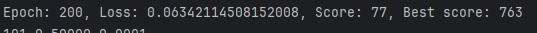
\includegraphics[width=13cm, height=1cm]{max-score.png}
    \end{center}

\section*{References}
\begin{enumerate}
    \item \href{https://sites.google.com/view/rbenchea/neural-networks}{Neural Networks Reference}
    \item \href{https://github.com/Farama-Foundation/Gymnasium}{Gymnasium Documentation}
    \item \href{https://github.com/Tavase/FlappyBirdGymnasium}{Flappy Bird Environment Repository}
    \item \href{https://pytorch.org/}{PyTorch Documentation}
\end{enumerate}

\end{document}
